\titre{20}
\theme{trigo}
\auteur{Nathan Scheinmann}
\niveau{1M}
\source{sesamath-1M-trigo}
\type{serie}
\piments{2}
\pts{}
\annee{2425}

\contenu{
	\tcblower
	\begin{minipage}[t]{0.45\textwidth}{
	\vspace{0pt}
	Soit un cercle de centre $C$ et de rayon $10$. Une corde $[BD]$ est regardée sous un angle de $20^\circ$ depuis un point $A$ du cercle. Calculer la longueur de la corde $[BD]$ et de l'arc $BD$. 	
	}
	\end{minipage}
	\hfill
	\begin{minipage}[t]{0.5\textwidth}{
	\vspace{0pt}
	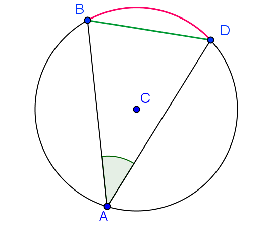
\includegraphics[scale=1]{../medias/1M/trigo/1M-exo-20}
	}
	\end{minipage}
}
\correction{

}

